\section{Introduction}
\label{sec:intro}

Search quality depends on both the graph index and the budget used to explore it. The index determines which paths a query can traverse, while the budget controls how much of that search is explored. HNSW and Vamana make this tradeoff central to efficient approximate nearest-neighbor search~\cite{malkov2020hnsw,subramanya2019diskann}. After rebuilding, a budget selected on the previous graph may execute on a different search structure. Preserving the parameter value does not establish that its recall behavior is preserved. This creates an operational question at the boundary between index maintenance and query serving: \emph{when can an existing budget policy be reused, and when is target-side information worth acquiring?}

The question has two distinct settings. Rebuilding an unchanged vector collection can alter the graph through construction order or randomization. Rebuilding after a data refresh additionally changes the collection and potentially the nearest-neighbor ground truth. Prior work documents construction sensitivity and develops efficient update mechanisms~\cite{elliott2024ordering,singh2021freshdiskann}. Adaptive search methods address another part of the problem: allocating work to individual queries using predicted recall or search cost~\cite{li2020laet,chatzakis2025darth,wang2026annie}. These capabilities make budget reuse attractive, but its value still depends on the relationship between the source calibration environment and the target index.

Evaluating that relationship requires more than comparing average recall. A policy can attain a high mean while a subset of queries falls below the requested quality. We study the probability that a query's recall is below a specified threshold, separately from the expected fraction of missed neighbors. In the primary experiment, failure means $\mathrm{Recall}@10<0.95$: because recall is discrete, even one missing neighbor is a failure. A 5\% risk target therefore asks that at least 95\% of queries recover all ten neighbors. This event is stricter than mean recall of 0.95 and must remain explicit when interpreting external methods.

Our organizing insight is that budget portability belongs to a \emph{source policy, target build, and query workload}. We call the resulting workflow \emph{Index-Conditioned Budget Audit} (ICBA). It records what information determines each action, separates target selection from certification and evaluation, and distinguishes absolute target failure from additional failure relative to a reference. The theoretical analysis is organized around the observation assumptions under which source information can or cannot support a target decision. The empirical analysis asks how often reuse fails, which evidence supports recovery, and what that recovery costs. \emph{Tiered Conformal Pooling} (TCP) provides the recovery case study: its history-pool replay reuses query-budget profiles and adjusts their decisions with target-selection information, followed by certification and fallback. The implemented first-passing pool and the assumptions needed for conformal coverage are distinguished in Section~\ref{sec:tcp-implementation}.

The primary replay covers SIFT-100K and Arxiv-Nomic-100K, with ten target builds per dataset after a 5\% mixed delete/insert refresh. Direct TCP pool reuse yields empirical target failure rates of \WZeroSiftSourceRisk\% and \WZeroArxivSourceRisk\%. Target-selection recalibration reduces them to \WZeroSiftTargetRisk\% and \WZeroArxivTargetRisk\%, while reducing mean distance calculations by \WZeroSiftTargetGain\% and \WZeroArxivTargetGain\% relative to the registered fixed endpoint. These results concern queries with corresponding old-build profiles; they measure empirical recovery in that replay population. Search savings and a valid certificate for the entire candidate/fallback decision are separate outcomes.

Figure~\ref{fig:overview} summarizes the operational question and the measured risk--cost tradeoff: direct reuse is cheap but exceeds the empirical risk target, whereas target recalibration retains a large part of the search savings.
\begin{figure*}[t]
\centering
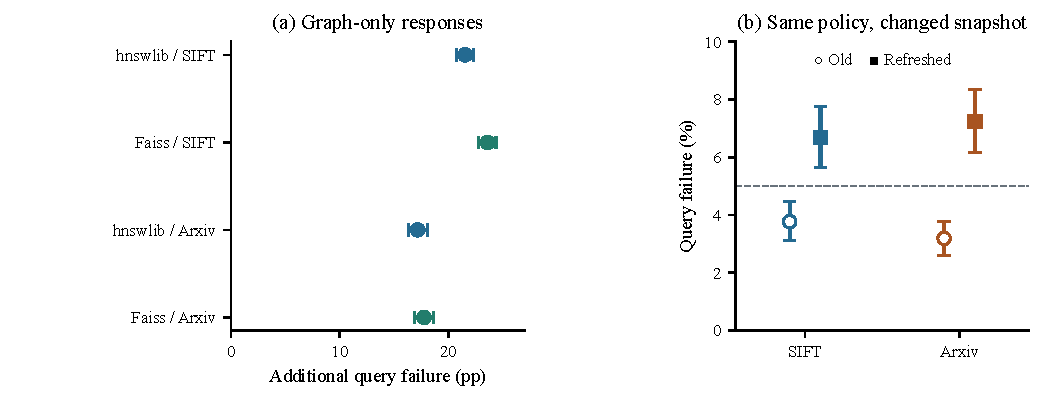
\includegraphics[width=\textwidth]{figures/overview.pdf}
\caption{Budget portability and the primary replay. (a) Schematic, not a measured graph: after refresh and rebuilding, an old query-budget profile is applied to a changed index. (b) Frozen two-dataset outcomes, averaged over ten target builds per dataset. Gain is relative to each dataset's fixed endpoint; recalibration includes fallback. The dashed line is the 5\% empirical risk target, not a confidence bound.}
\label{fig:overview}
\Description{A source-to-target index schematic and a scatter plot of empirical query failure versus mean distance-count gain. Direct reuse exceeds 5 percent failure; completed recalibration lies below it with approximately 44 percent gain on each dataset.}
\end{figure*}

\begin{table}[t]
\caption*{\textbf{Terms at a glance.} SIFT and Arxiv abbreviate SIFT-100K and Arxiv-Nomic-100K in tables and figures.}
\small
\begin{tabularx}{\linewidth}{@{}lX@{}}
\toprule
Term & Meaning in this paper \\
\midrule
ICBA & Index-Conditioned Budget Audit: the measurement and decision workflow. \\
TCP & Tiered Conformal Pooling: the history-based policy family; the primary replay uses a nine-history maximum and target grid shift. \\
NDC & Number of distance calculations; search work, not elapsed time. \\
CP / UCB & Clopper--Pearson / upper confidence bound. \\
Transport risk & Target failure of a transferred source policy, $\risk_{G_t}(\pi_s)$. \\
LOTO & Leave one target build out. \\
Endpoint & Largest registered action; its risk is measured, not assumed zero. \\
\bottomrule
\end{tabularx}
\end{table}

The broader evidence is deliberately layered. External-method bridges examine query-level risk under their supported interfaces, while Vamana and Deep1M analyses examine different graph-family and scale conditions. These blocks retain their own references and failure definitions. Recovery is then evaluated against its acquisition cost: obtaining target labels and profiles can outweigh cheaper searches over a short serving horizon. Thus, an operator needs both a risk assessment and an amortization calculation before replacing direct reuse with recalibration.

We make four contributions:
\begin{enumerate}
\item A build-conditioned formulation that separates absolute risk, reference-relative transfer loss, and the information available to the budget policy.
\item An ICBA audit workflow connecting query roles, discrete failure events, certification decisions, and search-cost accounting.
\item A layered empirical study of budget portability across the registered recovery, method-bridge, graph-family, and scale settings.
\item A TCP recovery case study that quantifies the search benefit of target information and its workload-dependent acquisition cost.
\end{enumerate}
Together, these contributions support treating the search policy as part of the index's versioned operational state, with an explicit decision about reuse after rebuilding.
